%!TEX root = doc.tex
\section{Comparison to Related Work} % (fold)
\label{sec:related_work}

Some works have approached the problem of complementing Repast and JADE's faults by bringing them together in a single framework by means of a middleware. In MISIA \cite{garcia2011misia} and JRep \cite{gormer2011jrep}, the authors' approach was successful in complementing Repast's and JADE's features, allowing them to create Repast simulations that also take advantage of JADE's networking capabilities and use of open standards.

MISIA's approach, as suggested by Figure \ref{fig:misia}, is to use a middle layer that acts as the bridge betweens the two other layers that interact with JADE and Repast S. By extending the representation of Repast and JADE agents and allowing them to communicate internally and to synchronize their state,
they work seamlessly as one.

\begin{figure}[h]
	\centering
	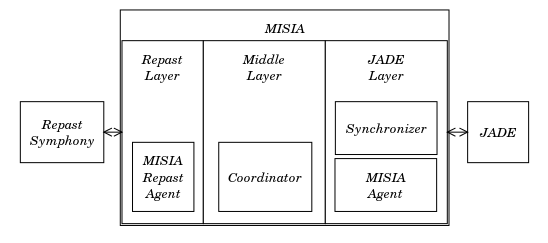
\includegraphics[width=0.5\textwidth]{figures/MISIA.png}
	\caption{Basic structure of MISIA. Diagram
		adapted from original paper. \cite{garcia2011misia}}
	\label{fig:misia}
\end{figure}

One of the challenges the authors iditified when re-implementing the FIPA interaction protocols was to synchronize them with Repast tick-based simulation. Given JADE's event-driven architecture, MISIA proposes the use of a coordinator agent that informs the JADE-Agent when a tick has passed. MISIA also proposes its own implementation of the interaction protocols supported by JADE, making them tick-friendly.

JReps's approach is not as complex as MISIA's. By having the Repast agent encapsulate the JADE agent representation, the synchronization is immediate and doesn't require an external coordinator. The two agent representations take care of synchronizing any state changes.

Each agent then takes care of interfacing their respective frameworks. The interaction between agents in JRep is performed with FIPA ACL; the protocols' implementation is provided by the JADE platform. Figure \ref{fig:jrep} represents the basic structure of this platform.

\begin{figure}[h]
	\centering
	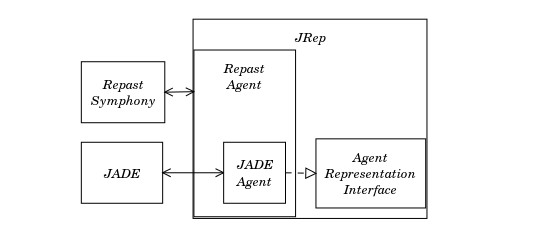
\includegraphics[width=0.5\textwidth]{figures/jrep.png}
	\caption{Basic structure of JRep. Diagram
		adapted from original paper. \cite{garcia2011misia}}
	\label{fig:jrep}
\end{figure}

The most obvious advantage of the approach proposed in this paper is the possibility of using Repast interaction protocols without the need to interface with JADE.

JADE is a very rich platform, but for many simulation scenarios, the overhead introduce by it will have an impact on the simulation performance. \cite{mengistu2008scalability} \apiname{}, as we describe with more detail in the next section, uses an implementation of those protocols that is conceptually very close to JADE's but tailored for Repast with no extra dependencies - in fact, the API could be used with other frameworks with little adaptation.

As suggested by Figure \ref{fig:related-repacl}, \apiname{}'s general structure is simpler than that of JRep and MISIA because, while these take advantage of both frameworks' features, \apiname{} is focused on the interaction protocols. Furthermore, unlike those, our proposal does not force the dual representation of agents in both frameworks.

\begin{figure}[h]
	\centering
	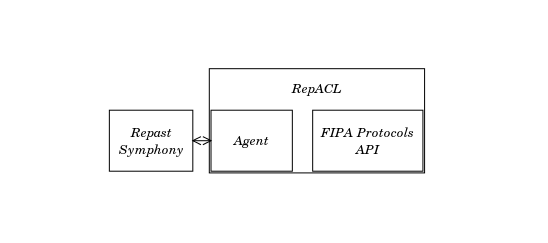
\includegraphics[width=0.5\textwidth]{figures/repacl.png}
	\caption{Basic structure of \apiname{} API}
	\label{fig:related-repacl}
\end{figure}
